%%%% fs-run-time-data-flow  FlameStream data flow

The key concept of \FlameStream\ model is a data stream. It is a sequence of discrete events described by data items, internally represented as 
$(Payload, Meta).$
The $Payload$ is processed by a user-defined code, while $Meta$ is handled with \FlameStream\ engine. In particular,
the primary purpose of the meta-information is to impose the total order on data items. 
The  $Meta$ is assigned at the entry (called {\em  front}) and is discarded at the {\em barrier} just before the exit. 

% \subsection{Computational flow}
The stream processing is specified by a logical execution graph. 
Each node of the graph represents a single operation on data items, and edges describe the routing of data items between operations.  
Our model allows cycles in the graph while such graphs are commonly assumed to be acyclic (DAGs) 
~\cite{Zaharia:2016:ASU:3013530.2934664, Carbone:2017:SMA:3137765.3137777}. 
The cycles are required for specification of certain computations (e.g. MapReduce-based) with our set of operation types (outlined below).
%Moreover, as we show further, there are cases when cycles are required, e.g., for MapReduce-based algorithms. 
Figure~\ref{logical-graph-figure} shows the example of logical execution graph.

% \subsection{Physical deployment and partitioning}
A distributed hardware environment is modeled as a set of {\em worker} processes. 
Each worker executes logical execution graph and has an assigned range of hash values used for physical routing of data items to workers. 
%An integer interval (hash range) is assigned to every worker. Intervals are not intersected and cover the range of 32-bit signed integer.
%
Each operation entry has a user-provided hash function called {\it balancing function}. This function is applied to the payload of data items and determines partitioning before each operation. After that, the data items are sent to the worker, which is responsible for the associated hash range. Therefore, load balancing explicitly depends on the user-defined balancing functions. 
%This allows the developer to determine optimal balancing which requires the knowledge of the payload distribution. The system optimizes the hash ranges assignment according to the processing statistics. 

\begin{figure}[ht]
  \centering
  \begin{minipage}[b]{.5\textwidth}
    \centering
    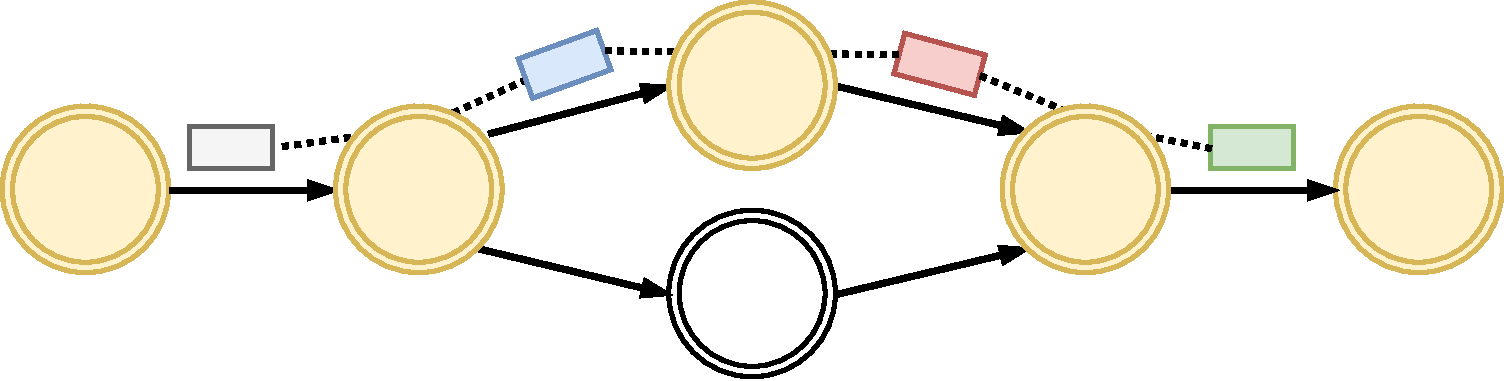
\includegraphics[width=0.9\linewidth]{pics/logical-graph}
    \caption{A logical execution  graph}
    \label{logical-graph-figure}
  \end{minipage}%
  \begin{minipage}[b]{.5\textwidth}
    \centering
    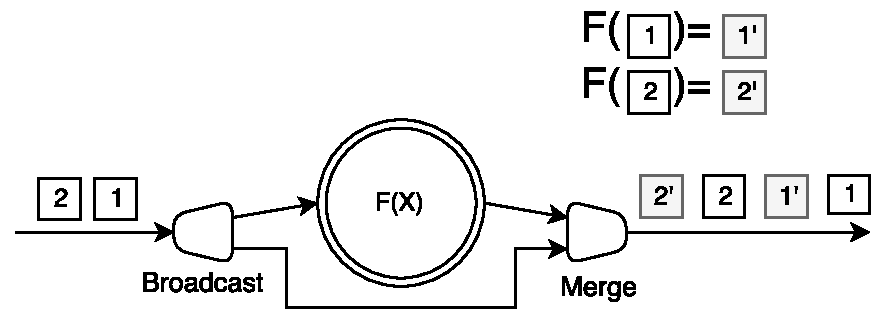
\includegraphics[width=\linewidth]{pics/ordering}
    \caption{The ordering model}
    \label{ordering}
  \end{minipage}
\end{figure}

% мм\subsection{Ordering model}

Data items are totally ordered according to labeles assigned to events at the entry as a part of meta-information. All operations preserve this order. Any additional items produced by an operation are placed between the item being processed and the next item. The ordering labels are dropped when items are delivered from the barrier. 

% We assume that there is a total order on data items. 
% Ordering is preserved when an item is going through the operations. 
% More precisely, the order of output items is the same as the order of corresponding input items. 
% If more than one item is generated, they are inserted in output stream sequentially. 
% Moreover, the output follows corresponding input but precedes the next item. 
% Without diving into details, it should be noted that the order of items is maintained across different fronts.

The ordering is illustrated  in Figure~\ref{ordering}. Data item with payload $1'$ is the derivative of the item with payload $1$, according to operation $F$. The same is for items with payloads $2'$ and $2$. After merge operation, the order between $1$ and $2$ is preserved. Furthermore, $1'$ follows $1$, and $2'$ follows $2$.  

%  We assume that input items of the operations are strictly ordered.

%  \subsection{Operations}

The list of available operations includes:
\begin {description}
\item [Map] applies a user-defined function to the payload of an input item and returns a (possibly empty) sequence of data items with transformed payloads. 

\item [Broadcast] replicates an input item to the specified number of operations.

\item [Merge] operation is initialized with the specified number of input nodes. It sends all incoming data to the output.

\item [Grouping] constructs a single item containing a set of consecutive items that have the same value of partition function. The maximum number of items that can be grouped is specified as a parameter  $Window Size.$ 

The output item of the grouping has the same ordering label as the last item in the output group. 
Groupings of different partitions are independent. 
Grouping is the only operation that has a state.

\end {description}

%has a {\it window size} parameter. Grouping stores input items into distinct buckets by the value of the input balancing function applied to the payload. When the next item arrives at the grouping, it is appended to the corresponding bucket. Each time the grouping outputs window-sized {\it tuple item}, which consists of the most recent (in terms of the meta-information) items of this bucket. If the size of the bucket is less than the window, all items of the bucket are taken. 

The following example illustrates  the grouping operation. 
Let the input stream be a series of integers: $ 1,2,3, \ldots$, and the  partition function returns for even numbers and 0 otherwise. If the window is set to 3, the output is 
$$(1), (2), (1|3), (2|4), (1|3|5), (2|4|6), (3|5|7), (4|6|8), \ldots$$

%The grouping operation has two important properties: the output tuple is identified by its last element, the results among items with different values of a partition function are independent.

% \subsection{User-defined parameters}

% A user can set up the following parameters:

% \begin{enumerate}
%  \item{Computational flow}
%  \item{Balancing functions of the inputs}
%  \item{Map functions}
%  \item{Grouping windows}
%\end{enumerate}

%These parameters can produce more than one graph, which can yield equivalent results. Choosing among them is a performance optimization problem that relies on the system.
%It is important to mention that there are no parameters for state-management. 
%Therefore, business-logic is stateless. Nevertheless, the operations set is enough to implement any MapReduce transformation as shown in the next section.

An important special case of grouping with $Window Size = 2$  provides for realization of stateful calculations with drifting state techniques manifested in section~\ref{motivation-section}.  
Indeed, consider a map operation that follows the grouping and sends its output to the grouping input. This map operation receives a pair of its previous output considered as the state object, and new incoming item from the source stream. The map operation calculates new state object and sends it back as the grouping input. 
More details are provided in the appendix~\ref{fs-drifting}.

% \subsection{Drifting state}

% Most of the computational pipelines require state carrying between consecutive data items. For example, moving average calculation needs partial sums to be stored. The state management in distributed systems is a complicated topic that requires delicate treatment. Some systems forces that all state management is put in business-logic: making state persistent, replication, ensuring state consistency, etc. Others shifts some difficulties to the system's concern, e.g., Flink provides a state API that guarantees consistency in case of failures \cite{Carbone:2017:SMA:3137765.3137777}.

%The core idea of {\it drifting state} is to fully integrate state management into the system internals by making a state a part of the heterogeneous data flow. 
% In order to do state updates, the drifting state is grouped with new elements, combined, and the new state is emitted. 
% WRONG!!!  The limited number of such combines can be implemented with DAG by repetition of grouping and map operations. 
%As stream processing is aimed to infinite sequences, there is a need for a cycle in the computational pipeline. 
%The exact structure of such cycle is described in appendix~\ref{fs-drifting} with an example of typical stateful transformation, MapReduce.

%The complex graph with multiple stateful operators can be constructed using a cycle for each stateful component. 
%It is important to say that such tangled structures may not be exposed to the end-user and can be hidden by some high-level API.

